\section{Preparación de los Datos}
Como se señaló en el Capítulo~\ref{ch:metodologia}, la preparación de los datos es la etapa más importante para la minería de datos. Durante este ca
\subsection{Creación de Indicadores}
En base a la revisión teórica en el Capitulo~\ref{ch:marcoteorico} se encontraron diferentes indicadores tentativos que son factibles para su creación.
A continuación presentaremos la creación de cada uno de estos en base a la entidad de dónde provienen. Además, todos los indicadores están relacionados a un alumno, en este caso, nuestras observaciones consisten en alumnos y nuestros campos o columnas, corresponden a los indicadores o características del alumno.
\cindicadores{MINEDUC}
\cindicadores{AgenciaDeCalidad}
\cindicadores{MIME}
\cindicadores{JUNAEB}
\cindicadores{CIAE}
\cindicadores{CIT}
\subsection{Preparación de la Muestra de Estudio}
Una vez terminada la creación de los indicadores obtenidos de diferentes conjuntos de datos, se necesitan realizar cruzamiento de los diferentes conjuntos de datos que contienen los indicadores.

Para lograr esto, utilizaremos Python y la librería Pandas que es capaz de trabajar con diferentes estructuras de datos entregando libertad al momento de juntar tablas.

\cuadro{6SolucionPropuesta/rconj}
En el Cuadro~\ref{tab:rconj} puede observar la cantidad de observaciones obtenidas por cada conjunto de datos en el Cuadro junto con los años disponibles de cada uno\footnote{Esto es válido también para los indicadores creados a partir de estos conjuntos de datos.}.

Lamentablemente como se puede ver en el Cuadro~\ref{tab:rconj} la disponibilidad de la totalidad de los conjuntos de datos es solamente para el año 2013, puesto tenemos la información geo-referenciada está disponible para ese año y solo para el Gran Santiago, además las encuestas SIMCE no permite asignarle esta información a todos los alumnos debido a que es solamente una muestra\footnote{No se sabe si es representativa o no del establecimiento, esto es algo que trataremos próximamente.}. Básicamente estas dos aristas limitan la cantidad de total de alumnos.

Todos estos conjuntos de datos con sus indicadores creados se deben juntar en una única muestra. Para lograr esto primero se crearán dos conjuntos de datos diferentes, esto lo logramos en tres etapas:\\
\begin{enumerate}[label=\Roman*]
\item \textbf{Preparación de conjunto de datos con identificador único MRUN} \hfill \\
Se cruzan todos los conjuntos de datos que contienen indicadores individualizados por el MRUN. Acá se obtiene la entidad 'Alumno' a través de varios cruzamientos de conjuntos de datos.
\cuadro{6SolucionPropuesta/cruceMRUN}
\item \textbf{Preparación de conjunto de datos con identificador único RBD} \hfill \\
Se cruzan todos los conjuntos de datos que contienen indicadores individualizados por el RBD. Acá se obtiene la entidad 'Establecimiento' a través de varios cruzamientos de conjuntos de datos. Además de los profesores se obtiene la entidad 'Docente' que está relacionada con los establecimientos.
\cuadro{6SolucionPropuesta/cruceRBD}
\item \textbf{Georefenciación de los conjuntos de datos} \hfill \\
Se utiliza la información del CIT para georefenciar a los alumnos y establecimientos con la finalidad de incluir información territorial a estos. Es decir, se agrega la entidad 'Manzana' a las otras entidades.
\end{enumerate}

\begin{figure}[H]
  \centering
    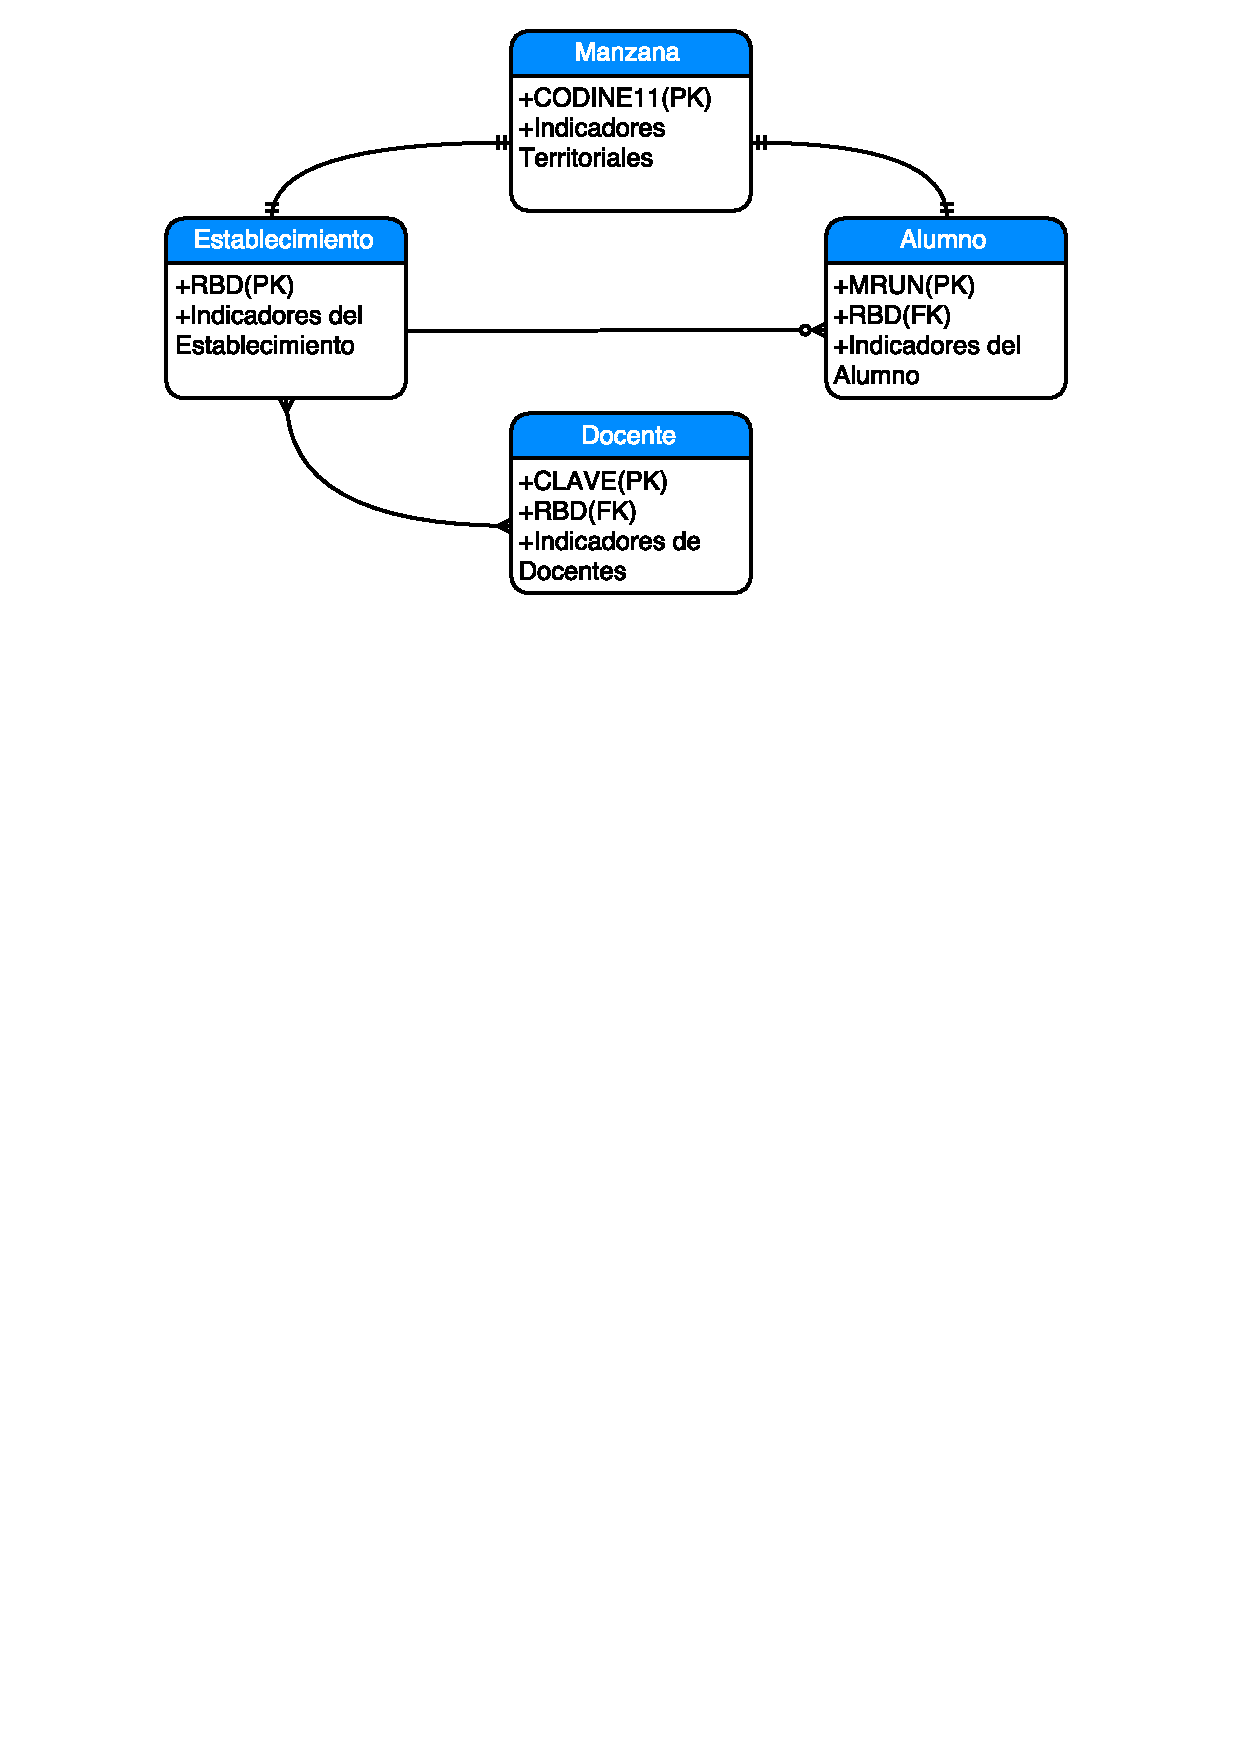
\includegraphics[trim=2cm 20cm 0cm 0cm,scale=0.9]{Figuras/6SolucionPropuesta/relacionDatos.pdf}
      \caption{Diagrama relacional de las diferentes entidades generadas.}
    \label{fig:rel}
\end{figure}

Se muestra en la Figura~\ref{fig:rel} las diferentes entidades 'Establecimiento', 'Alumno', 'Manzana' y 'Docente'.se obtienen dos conjuntos diferentes, uno sobre la información de los alumnos con georeferenciación y sus indicadores territoriales, y otro con información de establecimientos con indicadores territoriales también.

En la Figura~\ref{fig:venn} se presenta el diagrama de Venn\footnote{Representación gráfica de las relaciones existentes entre diferentes conjuntos} simplificado.para ver el resultado del procedimiento de cruzamiento de tablas\footnote{Este se hace a través de la función \textit{join} de Pandas que lo que hace es juntar dos tablas utilizando un índice especifico.}
\begin{figure}[H]
  \centering
    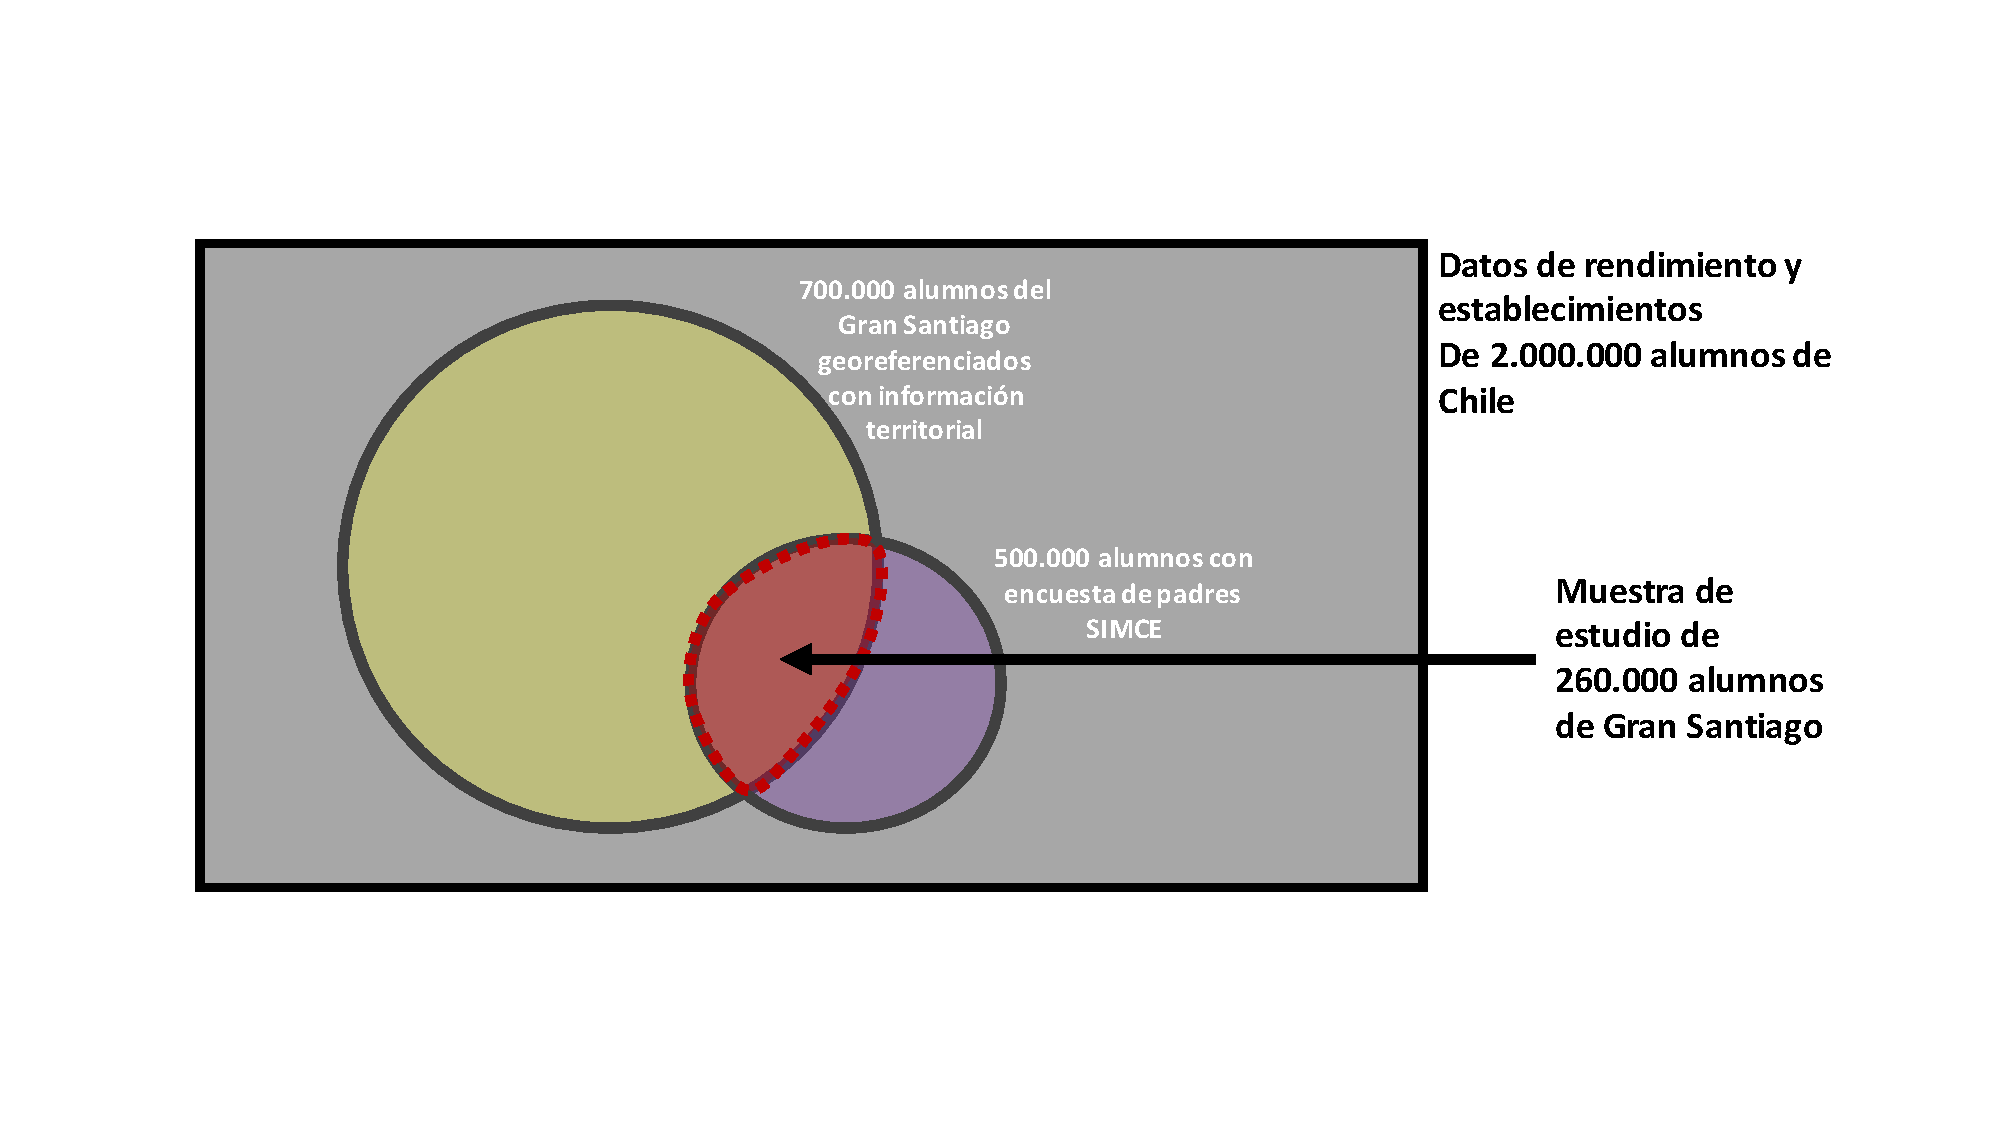
\includegraphics[trim=0cm 5cm 0cm 0cm,,scale=0.5]{Figuras/6SolucionPropuesta/Venn.pdf}
      \caption{Diagrama de Venn de la composición de la Muestra de Estudio}
    \label{fig:venn}
\end{figure}
Finalmente como vemos en la Figura~\ref{fig:venn} se obtiene una muestra de 260.000 estudiantes geo-referenciados del Gran Santiago con 93 columnas que representan indicadores o información de identificación de los alumnos.Desde ahora en adelante llamaremos variables a las columnas que no sean de identificación. Para ver un resumen del conjunto de datos y el libro de código, visitar el Anexo~\ref{an:muestra}
\subsection{Exploración y validación de la Muestra de Estudio}
Dado los problemas heredados del conjunto de datos de encuestas SIMCE estamos trabajando con una muestra de los alumnos de los establecimientos, no toda la población. Si bien la muestra representa aproximadamente un 30\% de la población de alumnos del Gran Santiago, debido a que el SIMCE no se da en todos los años es necesario hacer una revisión por grado de la tasa de deserción para evaluar la representatividad de la muestra obtenida. En la Figura~\ref{fig:deserciongradomuestra} se puede observar la distribución de la tasa de deserción por grado de la muestra Podemos notar que desde 3º Básico la tasa de deserción de la muestra se aproxima a la tasa de deserción de la población. Esto se puede explicar por que el SIMCE se da a partir de ese curso, por tanto es válido no tener alumnos de 1º básico a 2º básico. Entonces desde ahora, solamente vamos a trabajar con alumnos de 3º Básico a 4º Medio de establecimientos municipalizados y subvencionados del Gran Santiago.
Finalmente, al utilizar solamente alumnos de 3º Básico en adelante se eliminaron de la muestra aproximadamente $725$ alumnos, siendo marginal respecto al tamaño de la muestra total\footnote{Claramente, esto puede ser un factor que influyó en que la tasa de deserción esté distorsionada para esos grados.}


\subsection{Pre-procesamiento de la Muestra de Estudio}
En base a lo estudiado en el Capitulo~\ref{ch:marcoteorico} sabemos que para utilizar un algoritmo de aprendizaje automatizado se deben realizar diferentes procedimientos a los datos para que estos sean legibles para el algoritmo. El procedimiento de dos etapas que se le aplicará a las columnas disponibles\footnote{Para ver una lista de estas con su categorización por medida ver el Cuadro~\ref{tab:caract-var} en el Anexo~\ref{an:muestra}} que no sean de identificación son los siguientes:
\begin{enumerate}[label=\Roman*]
\item Separar variables de Índice de la muestra
\item Vectorización de variables nominales
\item Imputación de valores perdidos por variable\footnote{Para variables nominales se utilizó la mediana de los valores de la variable y para variables escalares se utilizó el promedio de los valores de la variable. }
\item Escalamiento uniforme entre un $-1$ y $1$ a variables de escala,nominales y ordinales.\footnote{La escala se calcula por variable, es decir, cada variable posee su escala 1 a -1 en función del valor máximo y mínimo respectivamente.}
\end{enumerate}

Una vez realizada esta última etapa, podemos proseguir con los siguientes pasos para poder lograr nuestro objetivo. Finalmente la muestra de estudio se compone de aproximadamente \textbf{260.000 alumnos del sistema regular escolar de escuelas municipales y subvencionadas de 3º Básico a 4º Medio del Gran Santiago}.


